\section{AutoLibra\protect
\includegraphics[height=1em]{figs/scale.png}}

\begin{figure}[!t]
    \centering
    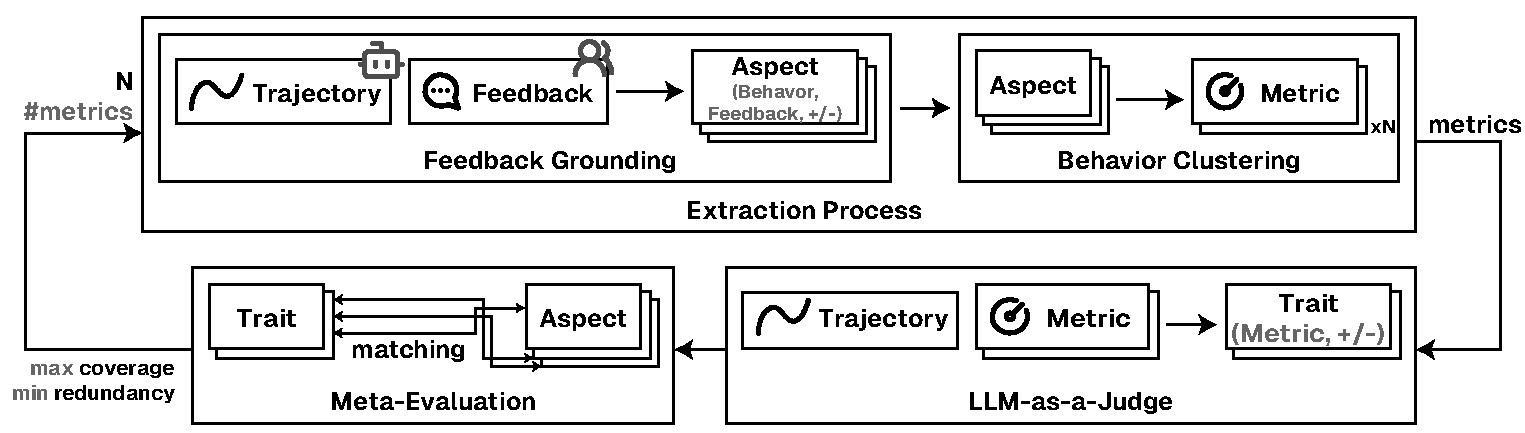
\includegraphics[width=\textwidth]{figs/autolibra-pipeline.pdf}
    \caption{AutoLibra pipeline. AutoLibra consists of three major components: Extraction Process
    turns annotated agent trajectories into metrics, LLM-as-a-Judge evaluates the agent trajectories
    based on the induced metrics, and Meta-Evaluation Process measures the quality of induced metrics
    through matching the detect agent traits with grounded feedback aspects.
    }
    \label{fig:autolibra-pipeline}
\end{figure}

To address the limitations of existing evaluation paradigms, we seek to design an evaluation method that 
meets the following desiderata: (1) \emph{data-driven}: this makes sure that the metrics are grounded
in the real agent behavior and human opinions, (2) \emph{generic}: applicable to various agent domains 
without the need for domain-specific design, (3) \emph{self-verifiable}: this provides guarantee that the 
induced metrics can be used in LLM-as-a-Judge to generate human-aligned evaluation. 

As illustrated in Fig. \ref{fig:autolibra-pipeline}, AutoLibra achieves these desiderata through a closed-loop pipeline
consisting of three major steps: \textbf{Extraction Process} first grounds the human feedback
for each trajectory into aspects (\S\ref{sec:grounding}), and then clusters the aspects into $N$ metrics (\S\ref{sec:clustering}).
\textbf{LLM-as-a-Judge} gives each trajectory scores for the induced metrics, the combinations of
metrics and scores becoming the traits of the agents (\S\ref{sec:llm-judge}).
Finally, \textbf{Meta-Evaluation Process} measures the quality of induced metrics through matching
the detected agent traits with aspects in the human feedback (\S\ref{sec:meta-evaluation}).
To optimize for the lowest redundancy with highest coverage, we control the number of metrics 
through a hyperparameter $N$ in the clustering step (\S\ref{sec:metric-optimization}). AutoLibra also supports
an interative metric induction process, where as the agent is optimized, new metrics can be addeding 
to the existing metrics (\S\ref{sec:iterative-induction}).

\subsection{Feedback grounding}
\label{sec:grounding}
The feedback of human annotators could contains multiple aspects, e.g. \textsf{AI agent was pretty good
on giving me a consistent itinerary and vacation plan, although It froze on the last couple of minutes.},
collected from human annotators in CoGym \citep{shao2024collaborative}, contains a positive aspect
about the agent's ability to generate a consistent itinerary, and a negative aspect about the agent freezing
at the end. Here we define an \emph{aspect} as a triple $(\texttt{behavior}, \texttt{feedback}, \texttt{sign})$.
In the positive aspect of the previous example, the \texttt{behavior} is the agent's actions to create
a 20-day itinerary for Maldives, the \texttt{feedback} is that the itinerary created is consistent, 
and the \texttt{sign} is positive. This grounding procedure is similar to coding in thematic analysis.

In this step, we not only feed the trajectory and feedback into the LLM (we use GPT-4o \citep{openai2024gpt4ocard} 
as it yields good results in our experiments), but also provide the LLM with the following instructions:
(1) break down the feedback into bulletpoints; (2) for each bulletpoint, find the corresponding
part of the trajectory that the feedback is referring to. Finally, we use constrained decoding to force GPT-4o
to output the aspects in the previous format. In our experiments, we find that on most datasets, for each
trajectory, the LLM can generate one to five aspects, with an average number of one to two aspects per trajectory.


\subsection{Behavior clustering}
\label{sec:clustering}

The second step of the Extraction Process is to cluster the aspects into $N$ metrics.
To illustrate this step, we consider another example in the same dataset
\textsf{The AI responds quickly to write and run the Python script.} where
the \texttt{behavior} is the agent's action to quickly write and run a Python script, the \texttt{feedback}
is that the agent responds quickly, and the \texttt{sign} is positive. Although this aspect is a positive aspect,
it reflects the same dimension of the agent's behavior as the previous negative aspect just on the opposite side.
Each \emph{metric} is a cluster of aspects, with a definition summarizing the criteria of positive behaviors,
and a list of positive behavior examples, and a list of negative behavior examples. This clustering procedure
is similar to the theme induction step in thematic analysis.

However, clustering similar agent behaviors together is challenging for statitiscal clustering methods.\footnote{
    In preliminary experiments, we tried to use K-means clustering on the aspect vectors generated by \texttt{text-embedding-3-large},
    but the clusters are mostly based on tasks and not on the behaviors.
}
Inspired by \citet{viswanathan2024large,lam2024concept}, we prompt an LLM
(
    we use o3-mini high\footnote{https://openai.com/index/openai-o3-mini/}, as it yields the best coverage and redundancy scores
    as evaluated later
) to cluster the aspects 
into $N$ metrics, and provide the LLM with the following instructions:
The granularity of the grouping should be minimal, only very similar behaviors should be grouped together.
But don't limit to one particular website or one particular character.


\subsection{LLM-as-a-Judge}
\label{sec:llm-judge}

LLM-as-a-Judge \citep{zheng2023judging},
or more broadly model-based evaluation 
\citep{zhang2019bertscore,celikyilmaz2021evaluationtextgenerationsurvey}
is a method to rely on machine learning models to evaluate the output of other machine learning models.
The success of it depends on the gap between the difficulty of the evaluation or verification and 
that of generation and action. 
In agentic tasks, this gap is often large, as the policy model needs to perform 
multiple steps of decision making, while the evaluation model only needs to
classify the trajectories, which make LLM-as-a-Judge widely used \citep{zhouwebarena,he2024webvoyager,zhousotopia}.
In AutoLibra, we also use LLM-as-a-Judge as the evaluation method to
evluate the agent trajectories based on the induced metrics. However, LLM-as-a-Judge
can be replaced by any other evaluation methods implementing the induced metrics,
e.g. \texttt{interact-valid-element} metric
could be evaluated by a rule-based evaluator which checks if the agent
interacts with valid elements on the webpage. Future research could explore
programmtical evaluation generation methods \citep{maeureka} to generate 
programs for the induced metrics.

Taking the induced metrics as input, an LLM (we use o3-mini medium,
as it provides similar results in this step as o3-mini high
but is cheaper to run) is prompted to rate agent trajectories into
\{+1, -1, N/A\} for each metric. The output of LLM-as-a-Judge is a set of
positive \emph{traits}, and a set of negative \emph{traits}. When we calculate the scores of 
the metrics, we use the ratio of agent trajectories rated as positive
to the ones that are rated as positive or negative, ignoring the N/A ones,
since not all metrics are applicable to all trajectories ---
some metrics like \texttt{valid-search-terms} are only applicable when the task
involves searching. 

\subsection{Meta-evaluation}
\label{sec:meta-evaluation}

The last component of the loop is the Meta-Evaluation Process. ``Meta'' here implies 
that we are evaluating the evaluation metrics and results. 
This step takes the traits and the aspects in the 

\subsection{Metric optimization}
\label{sec:metric-optimization}

\subsection{Iterative metric induction}
\label{sec:iterative-induction}